\chapter{The Flexibility Stack}
\label{ch:stack}

Picture an operator in West Texas with two documents on their desk. One is next year's power contract, unsigned, from a retail supplier who will sell at the real-time index, at a fixed price, or at a fixed price with the right to sell back. The other is a letter from the wind farm across the road, offering power behind the fence at a price no retail supplier can match, on the condition that the mine gives up most of what this part of the book has been pricing. Five chapters have priced the pieces of that decision one at a time. This chapter prices them together, for one site, over five years of real prices, and answers the four questions the operator actually has: which contract to sign, which layers of flexibility to switch on and in what order, what the whole stack is worth against simply running the machines, and whether to take the fence instead.

\section{One Site, Five Markets}
\label{sec:stack-site}

The site is built from Chapter~4's two machines, so that every number in the earlier chapters carries over unchanged: 10,000 Antminer S19j~Pro at 104~TH/s and 3,068~W, and 10,000 Antminer S21~XP at 270~TH/s and 3,645~W, together 67.13~MW and 3.74~EH/s at stock power. % src: analysis/checks/ch9_flexibility_stack.R console "The reference fleet" (30.68 + 36.45 MW; 1.04 + 2.70 EH/s)
Run flat out at the power ceilings of Chapter~5, 3,420 and 3,990~W, it would draw 74.10~MW. Both totals are the machines' own draw, under the 75~MW line at which a site becomes a Large Load in ERCOT's rulebook, so neither batch-study route of Chapter~3 applies to it. That line counts the whole site at its meter, and the ledger simplifies by assuming the site draws nothing beyond its machines. A real site, with Chapter~1's tenth more for cooling and transformer losses, would have to hold its machines to about 68~MW, near stock power, to stay under it. Senate Bill~6 also lets the commission lower the threshold its own rules use \autocite{texas2025sb6}. The minimum billing demand of the commission's 12CP proposal (Section~\ref{sec:twelvecp}) would not reach a site that stays under that line, so the peak game of Chapter~8 is still open to it, and this chapter is a design brief for such a site. % src: analysis/checks/ch9_tuning.R header (ceilings 3,420 and 3,990 W: 34.20 + 39.90 = 74.10 MW); chapter 3 sec:miners-ercot; chapter 8 sec:twelvecp; the line counts the whole site: ercot2026protocols sec. 2 (Large Load, "One or more Facilities at a single site with an aggregate peak Demand greater than or equal to 75 MW behind one or more common Points of Interconnection (POIs) or Service Delivery Points") and puct2026order58481 25.194(c)(14), order p. 227 ("total expected non-coincident peak demand at a single site is equal to or exceeds 75 MW"), while 74.10 MW is the machines alone; at the meter, chapter-1.tex:116 (CBECI2026 PUE 1.10, a tenth more than the machines): 67.13 x 1.10 = 73.84 MW at stock power, 74.10 x 1.10 = 81.51 MW flat out, and 75 / 1.10 = 68.18 MW of machines at most; texas2025sb6 sec. 2, PURA 37.0561(c) ("a demand threshold of 75 megawatts unless the commission determines that a lower threshold is necessary"); puct25205 adoption preamble (a 25 MW threshold declined, April 2026); the batch-study routes are elections for a Large Load in Batch Zero only: ercot2026protocols sec. 23 Form W (July 11, 2026: an ILLE "with a Large Load interconnection request eligible for study in the Batch Zero Process may elect" PCLR evaluation; "PCLRs are not eligible to qualify to provide Ancillary Services to the ERCOT System") and ercotplanningguide2026 secs. 9.2.2.1-9.2.2.2 (Forms W and X), as chapter 3 sec:miners-ercot prints; registration (EXEC-030, not printed): the ledger sells only RRS, ECRS and Non-Spin (analysis/checks/ch9_optimal_stack.R PRODUCTS), all open to a Load Resource that is not a CLR (ercot2026protocols sec. 3.6.1(1)(a)(iii)-(v); only Regulation, (i)-(ii), needs a CLR), so the site needs no CLR registration and no PCLR route; NPRR1188's gray box in sec. 3.6.1(5) moves only a CLR that is not an ALR to its Resource Node Settlement Point, so the site keeps the LZ_WEST price; the five ledger years also precede NPRR1188 (scheduled early 2027, chapter 3 sec:dam-rtm), when every load settled at its zone; reserve clearing prices are system-wide (analysis/data/ercot_dam_as_mcpc.csv.gz: one price per product per hour, regdn, regup, rrs, nspin, ecrs), so no Part III reserve revenue depends on node versus zone, even for a CLR; only energy-side figures priced at LZ_WEST (strike gains, adders) would change for a site settled at its node after 2027
It connects at LZ\_WEST, the zone Chapters~5 and~6 priced, and buys on the real-time index unless a section says otherwise. The S21~XP is a 2024 machine and the S19j~Pro reached the market later in 2021, after the storm, so the fleet is a control held fixed across the five years, and the early columns of every table answer what today's fleet would have earned in those markets, not what a site of the time did \autocite{bitmain2021s19jpro,bitmain2024s21xp}. % src: Bitmain specification pages (S19j Pro, 2021; S21 XP, 2024), as cited in chapter 4

The five years are five different markets, and the book has met each of them. 2021 is the storm year: Winter Storm Uri in February, real-time prices at the cap for days, the case study of Chapter~2. 2022 is the hangover, gas-driven prices with no emergency. 2023 is the ECRS year, when a new reserve product launched in June and spent its first year as the most expensive on the board, Chapter~7's story. 2024 is the flood, when batteries emptied the reserve markets and flattened the daily price spread, Chapter~6's story and Chapter~7's. 2025 is the threshold, the last year priced almost entirely by the old market; RTC+B went live in its final month. % src: chapter 2 (Uri); chapter 7 fig:as-history caption (ECRS June 2023, batteries, RTC+B December 2025); chapter 6 sec:batteries

Across those years the market changed, and so did the miner; the second change matters as much as the first. Chapter~4's identity, revenue per megawatt-hour consumed equals hashprice times 41,667 divided by efficiency in joules per terahash, makes the pause threshold follow hashprice, and hashprice fell six-fold: from \$0.310 per terahash-day in 2021 to \$0.051 in 2025 on the companion repository's spliced series. So the S19j~Pro's strike ran about \$440 in 2021, then \$172, \$104, \$90 and \$72, and the S21~XP's from about \$960 to \$157. % src: analysis/checks/ch9_flexibility_stack.R console "The strike moves with hashprice" (S19j Pro $439 / $172 / $104 / $90 / $72; S21 XP $958 / $376 / $228 / $198 / $157; hashprice $0.31049 -> $0.05078); series analysis/data/hashprice_daily_2021on.csv (usd_th_day_spliced), built by analysis/data/fetch_hashprice_history.py, its ten missing days filled by analysis/checks/ch9_hashprice.R
A \$440 strike pauses only in a catastrophe. A \$70 strike pauses on an ordinary summer evening. Chapter~6 priced the strike for 2025; this chapter prices five different games, each with its own strike, because holding the 2025 strike fixed across the years would ask a rosier question, and the wrong one. Table~\ref{tab:stack-markets} lays the five years side by side.

\begin{table}[htbp]
  \centering
  \scriptsize
  \setlength{\tabcolsep}{2.2pt}
  \begin{tabular}{lrrr>{\raggedright\arraybackslash}p{2.5cm}r>{\raggedright\arraybackslash}p{1.8cm}}
    \hline
    \textbf{Year} & \textbf{Hashprice} & \textbf{Strike} & \textbf{Zone} & \textbf{Best reserve vs.\ strike} & \textbf{Peaks} & \textbf{Best in hindsight} \\
     & \$/TH/day & S19j / S21 & mean & \$ per MW-year & by strike & \\
    \hline
    2021 & 0.310 & 439 / 958 & 148 & RRS 2,735,205 vs.\ 950,401 & 0 of 4 & reserves, window skipped \\
    2022 & 0.122 & 172 / 376 & 62 & Non-Spin 196,973 vs.\ 120,344 & 1 of 4 & strike, target, window \\
    2023 & 0.074 & 104 / 228 & 59 & ECRS 286,136 vs.\ 217,602 & 3 / 2 of 4 & reserves, window \\
    2024 & 0.064 & 90 / 198 & 36 & ECRS 72,308 vs.\ 45,918 & 0 of 4 & strike, target, window \\
    2025 & 0.051 & 72 / 157 & 42 & Non-Spin 26,699 vs.\ 45,983 & 0 of 4 & strike, target, window \\
    \hline
  \end{tabular}
  \caption{Five markets, one site. Hashprice is the annual mean of the spliced daily series; the strike is hashprice times 41,667 divided by 29.5 and 13.5~J/TH; the zone mean is the mean LZ\_WEST real-time settlement point price in \$/MWh. The reserve column compares the year's best standing revenue per megawatt-year, Chapter~7's ceiling, with what the same megawatt of S19j~Pro earned from the strike alone. ``Peaks'' counts the official 4CP intervals the strike would have paused on its own, S19j / S21 where the fleets differ. The last column is the hindsight ceiling of Section~\ref{sec:stack-sum}, which weighs reserves against the strike and the power target with the year's own outcomes in hand. It is a ceiling, not a plan: the site an operator could have planned in advance differs from it in four years of five.} % tab-src: analysis/checks/ch9_flexibility_stack.R console (strike section, Layer 2, Layer 3 coverage lines: S19j Pro 0/1/3/0/0 of 4, S21 XP 0/1/2/0/0 of 4); analysis/checks/ch9_optimal_stack.R console (HINDSIGHT CEILING and PLANNED lines; planned differs from hindsight in 2021, 2022, 2023, 2024)
  \label{tab:stack-markets}
\end{table}

The block of hours Chapter~8 tested as its second rule, weekdays from 4 to 6~p.m.\ in June through September, is called the \glossaryterm{summer-window}{summer window} from here on. % src: analysis/checks/ch8_4cp_rules.R, rule B (weekdays 16:00-18:00 Central, June-September), defined in chapter 8 sec:fourcp-rules

The ledger conventions are stated once and hold everywhere. The loop decides each quarter-hour on the last published settlement point price (a slower feed than Chapter~5's five-minute prints) and on the previous day's hashprice, because a day's network revenue is not known until the day closes; it books revenue and cost at what actually settled; a perfect-foresight twin runs alongside so that every line can state the price of not seeing the future. The loop treats each settled price as readable the moment its quarter closes; through ERCOT's public API it arrives a median 4.8~minutes later, on the same poll as Chapter~5's prints. Deciding a full quarter-hour late would have cost the planned site \$1.1~million of its \$123~million over five years, and the measured delay is about a third of a quarter-hour. The same discipline holds one level up, for the two switches a site sets once a year, which fleets hold reserve awards and whether to play the summer window: the planned case sets them as an operator could have, in advance, and the hindsight ceiling is printed beside it, never as a plan (Section~\ref{sec:stack-sum}). No forecast of any kind appears. Every dollar in this chapter's ledger is printed by one of two scripts in the companion repository, and the two checks on that ledger by two more; the historical calculator in the same repository runs the same engine, so the reader can rerun the grid site's ledger that follows with a different mix of the two machines, in one of four zones or under one of five contracts. The ledger's stock point is the measured curve's, 28.5 and 12.8~J/TH rather than the nameplate 29.5 and 13.5 of Sections~\ref{sec:stack-contract} and~\ref{sec:stack-strike}, which lifts its pause threshold about 3 and 6 percent, so its strike line runs 1 to 5 percent below the per-megawatt figures quoted there, and the two bases do not add up exactly. % src: analysis/checks/ch9_flexibility_stack.R header (lag conventions; p_lag, the previous 15-minute settlement price); chapter 5's loop decides on the NP6-788 five-minute prints, one print late (analysis/ch5-backtest/mixed_basis_study.py, whose slow feed is the first print of each settlement interval, not the settlement price); analysis/checks/ch9_optimal_stack.R header (curve stock point 28.57 / 12.76 J/TH on the 100 W grid; telemetry 28.48 / 12.81 at 3,068 / 3,645 W); checks: analysis/checks/ch9_control_friction.R and ch9_vs_papo.R; analysis/checks/ch9_calculator_export.R (calculator payload from the same functions, on the ledger's basis, the power target solved on S21 XP shares of units 5 percent apart and interpolated; analysis/calculator/ch9_calculator.html; analysis/calculator/check_calculator.mjs holds the page, for this site, to analysis/data/ch9_optimal_stack.csv to the dollar in every year; its ZONES are LZ_WEST, LZ_NORTH, LZ_HOUSTON and LZ_SOUTH and its CONTRACTS the five of sec:stack-contract; it has no fence, indifference price, ERS or RTC+B buyout, so it stops before sec:stack-fence); strike price ratio 29.5/28.574 = +3.2% and 13.5/12.757 = +5.8%; ledger strike_gain (analysis/data/ch9_optimal_stack.csv) $59.79/6.61/12.73/2.19/1.89M against sec 9.3's per-MW figures grossed to 30.68 and 36.45 MW, $60.31/6.76/12.90/2.28/1.99M (the stack console's strike column), i.e. 0.8/2.3/1.3/3.9/5.2% below; both book the pauses the lagged rule got wrong at what they cost, the stack script since 2026-09-27 (it clipped them at zero before, when the gap was 1.2 to 12.0%); readability: analysis/checks/ch5_api_readability.py console, NP6-905 full window median 287.0 s after the interval ends (4.78 min, n=818, 30.6% later than five minutes); lag sensitivity: CH9_LAG_Q=2 Rscript analysis/checks/ch9_optimal_stack.R, "flexibility over never pausing, 2021-2025: planned $122.33M" against $123.46M at the default (-$1.125M; by year 2021 -0.319, 2022 0, 2023 -0.638, 2024 0, 2025 -0.168; never-pause, the annual reserve and window choices and the hindsight picks unchanged; CH9_LAG_Q=3 gives $121.31M). The 287 s is 0.32 of a quarter-hour
Each ledger year is the whole calendar year, every quarter-hour of it, with one exception: 2021 starts on January~2, the first day with a previous day's hashprice to decide on. % src: analysis/checks/ch9_hashprice.R (ch9_check_calendar stops the run on any missing date or quarter-hour; the ten days missing from the spliced hashprice series, 2025-11-13 to 15 and 2026-08-17 to 23, filled from analysis/data/hashprice_daily.csv, which equals the spliced column on all 957 shared days); ch9_optimal_stack.R console header line ("2021 starts on 2021-01-02"; 8,736 h in 2021, 8,760 in 2025)

Two comparators run through the chapter. The first is the \glossaryterm{never-pausing-site}{never-pausing site}: the same fleet at stock power in every interval, present at all four summer peaks, paying every line of the ledger Chapter~6 built in Table~\ref{tab:btm-ledger}: losses, the ancillary and uplift allocations, the distribution line, and the whole transmission charge. It is the site that does not use its flexibility, and every gain in this chapter is measured against it. The second is the fence, the behind-the-meter site of Section~\ref{sec:btm}, which waits until Section~\ref{sec:stack-fence}. One word is fixed too. \emph{Curtailment} is the industry's word for the load coming off, whoever triggers it; where this chapter needs to say the machine stopped on its own rule, it says \emph{pause}.

\section{The Contract Decides the Baseline, Not the Option}
\label{sec:stack-contract}

Chapter~6 made a claim at the scale of one megawatt (Section~\ref{sec:arbitrage}): flexibility pays the same dollars under every contract that permits it, and only the baseline moves. At the scale of the site, over five years, the claim holds to the dollar. On the real-time index the S19j~Pro fleet's pause option was worth \$1.41~million in 2025; under a fixed \$27 contract with the right to sell back, \$1.41~million; under Riot's Corsicana price of \$43.95 with sell-back, \$1.41~million. What moved was the never-pausing baseline, from \$7.9~million on the index to \$12.0~million at a fixed \$27, because \$27 sat below the year's \$42 average. % src: analysis/checks/ch9_flexibility_stack.R console, Layer 1, S19j Pro 2025 rows: rt_index 7.94 -> 9.35; fixed_sellback 12.02 -> 13.43; ppa_sellback 7.47 -> 8.88; take-or-pay 12.02 flat; the lagged gain is $1,410,763 on all three, one engine; before 2026-09-27 the script clipped wrong pauses at zero and printed 9.44 / 13.52 / 8.96
The one shape that destroys the option is the one Chapter~6 warned about. A fixed take-or-pay contract without resale earned exactly nothing from flexibility in every one of the five years, on both machines: the reflex is intact, the contract has cut its wire. % src: ch9_flexibility_stack.R Layer 1, "Fixed $27 take-or-pay" rows: uplift 0.0% in every year for both fleets
Such a site can still physically pause for a summer peak, but it forfeits the whole value of the megawatt-hour instead of the spread between that value and the price, so the peak layer is crippled along with the strike.

The second lesson concerns the choice of index. The day-ahead site has the easier job of the two: its price is posted the afternoon before, so its loop is never late on the price at all, and it captured better than 99.7~percent of perfect foresight in every one of the five years, against the real-time site's 79 to 99. It still finished behind every time. On total margin before grid charges the real-time index won in all five years on both fleets, by \$8,100 to \$55,000 per megawatt-year. % src: ch9_flexibility_stack.R Layer 1 capture column: dam 99.7-100.0% every year both fleets, rt 79-99% (S19j Pro 99 / 92 / 92 / 84 / 89, S21 XP 99 / 90 / 87 / 79 / 86); total profit per MW-yr, rt less dam: S19j Pro 13,895 / 51,843 / 26,090 / 10,088 / 15,962, S21 XP 10,029 / 54,801 / 30,100 / 8,128 / 13,908 (console block "Real-time index less day-ahead index")
The reason is the price, not the loop, and it has two parts that take turns. The Day-Ahead Market clears once, on forecasts, while the scarcity that pauses respond to appears only in the real-time prints, so the spikes a day-ahead site would have paused on were never in its price. And the day-ahead average usually lands above the real-time one, by a difference realized after the year closes rather than quoted in advance, and not a fixed one: its annual mean ran 2.1~percent below the real-time mean in 2021, then 2.4, 8.8, 3.4 and 1.3~percent above it. % src: ch9_flexibility_stack.R console block "Real-time index less day-ahead index" (DAM - RT: -2.13% / +2.37% / +8.84% / +3.38% / +1.28%, LZ_WEST annual means of analysis/data/ercot_dam_spp_loadzones_2021on.csv.gz against ercot_rtm15_spp_loadzones_2021on.csv.gz)
In 2021 the day-ahead site bought cheaper and still lost, because the missing spikes were worth more than the discount; in 2022 and 2025 the missing spikes again did most of the work; in 2023 and 2024 the difference carried the result, and in both the day-ahead site's pause option was actually worth more. % src: same block, per MW-yr baseline + option = total: S19j Pro 2021 -27,600 + 41,495; 2022 12,947 + 38,896; 2023 46,021 - 19,931; 2024 10,611 - 523; 2025 4,735 + 11,227 (S21 XP the same baseline, option 37,630 / 41,854 / -15,921 / -2,483 / 9,173)
Perfect information about the wrong number is worth less than a late look at the right one. If you index, index real time.

The retail adder and the fixed-price forward curve are private, as Chapter~6 said, so the fixed prices above are the two the SEC filings disclosed, used as labeled scenarios. And Chapter~6's \$49,000 per megawatt-year for the S19j~Pro's strike in Figure~\ref{fig:strike-sweep} was a fixed-strike, same-interval figure: one strike of \$72 for the whole year, and the option priced with the interval's own settlement price. The executable version, priced with each day's own strike and decided one settlement interval late, comes to about \$46,000. Two things moved. Letting the strike float with hashprice adds about 5~percent, to the \$51,000 Section~\ref{sec:ownergen} already reported; deciding one settlement interval late takes about 11~percent back, the 89~percent capture above. % src: analysis/figures/fig_ch6_strike.R console ($49,116 per MW-yr at a fixed $71.6 strike); analysis/checks/sell_vs_mine.R moving-strike table (2025 $51,499 per MW-yr, same-interval), equal to ch9_flexibility_stack.R 2025 S19j Pro foresight gain 1,579,982 / 30.68 MW = $51,499 on the same full calendar; ch9_flexibility_stack.R Layer 2, 2025 "strike S19j" $45,983 (lagged, a late pause into a cheap interval booked at its loss, as ch6_strike_events.R books it) = 1,410,763 / 30.68 MW; 51,499 / 49,116 = +4.9%; 45,983 / 51,499 = 89.3%; until 2026-09-27 the script clipped those losses at zero and printed $48,730 (94.6%)
That 11~percent is the price of not seeing the future for a site that only pauses, at stock power, on the last settlement point price. From 2025 to mid-2026, Chapter~5's loop, deciding on five-minute prints, paid about 1 to 2 points of its capture for the same blindness, but against an oracle that also moves the power target, so the two figures do not compare one for one. % src: analysis/ch5-backtest/capture_anatomy.py console, TEST-2025-26 (2025-01-01 to 2026-06-22 Central, LZ_WEST), "INFO shortfall ... = information ... + friction": information, 100 minus the capture of a frictionless loop deciding on print i-1, is 0.97 (S21 XP) and 2.19 (S19j Pro) capture points, basis 0.71 and 1.49 (no print reveals the settlement point price) plus latency 0.27 and 0.70 (one print late); "INFO frictionless causal loop" 99.03 and 97.81; graded against chapter 5's oracle, which also moves the power target, not against this chapter's stock-power, pause-only twin (ch9_flexibility_stack.R gain_fc); in 2024 information is 2.48 and 5.58, hence the window
Across fleets and years, deciding late cost 1 to 21~percent. That is the first of two caveats on this chapter's price-only figures. % src: ch9_flexibility_stack.R console, "The price of not seeing the future" (real-time index), 1 - lagged/foresight: S19j Pro 0.8 / 8.3 / 8.4 / 16.2 / 10.7%, S21 XP 0.6 / 10.1 / 12.6 / 20.9 / 14.0% (2021-2025), the Layer 1 capture column's 79-99%; the 11 percent is the S19j Pro's 2025 cell; until 2026-10-04 this line said "The 11 percent is the first of two hedges this chapter carries in every number it prints", one fleet-year's gap applied to every number, reserves and baselines included

\section{Layer One: The Strike, Executed}
\label{sec:stack-strike}

Priced with each year's own strike and a lagged loop, the pause option is a scarcity-year instrument that pays a thin premium in ordinary years. For the S19j~Pro on the real-time index it was worth about \$950,000 per megawatt-year in 2021, then \$120,000, \$218,000, \$46,000 and \$46,000. For the S21~XP, whose strike sat higher still, about \$855,000 and then \$84,000, \$171,000, \$24,000 and \$16,000. % src: ch9_flexibility_stack.R console, Layer 2 table, "strike S19j" and "strike S21" columns (950,401 / 120,344 / 217,602 / 45,918 / 45,983; 854,511 / 84,195 / 170,877 / 23,956 / 15,938 per MW-yr)
Chapter~6 priced the same option from the other side of the fence, as the owner's right to sell, and found that almost all of 2021's value fell in the one week of the storm: 94~percent of it in Section~\ref{sec:ownergen}'s same-interval version. The executable version is no different in shape. The strike is an option: its value sat in one week of 2021 and one summer of 2023, and it was thin in 2024 and 2025.

\begin{figure}[htbp]
  \centering
  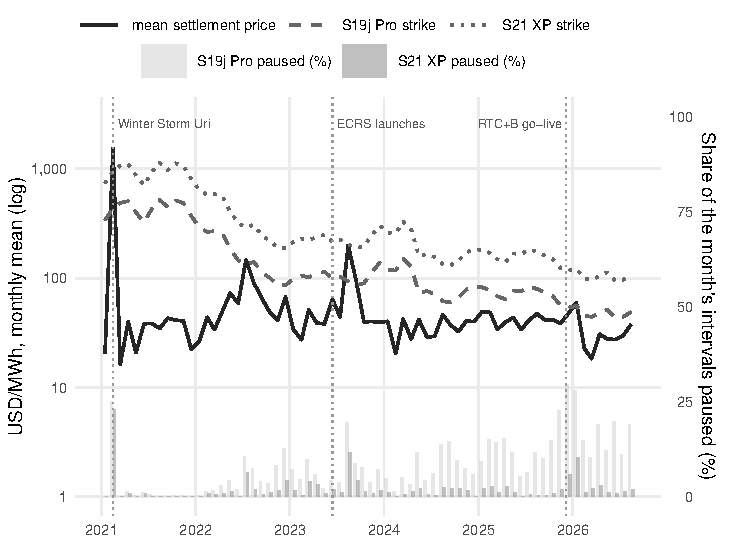
\includegraphics[width=\textwidth]{images/ch9_moving_strike}
  \caption{Five markets, two strikes, and the first months after. Monthly means of the LZ\_WEST real-time settlement point price and of the two machines' strikes, January 2021 to August 2026, on a log scale; the bars are the share of each month's quarter-hours the lagged rule paused each fleet. In 2021 the strikes floated far above every price but Uri's; by 2025 the S19j~Pro's averaged \$72 against a mean price of \$42, close enough that the fleet paused 14~percent of the year; in the eight months of 2026 under RTC+B it paused 17~percent. Strike = hashprice $\times$ 41,667 $\div$ J/TH, at 29.5~J/TH (S19j~Pro) and 13.5~J/TH (S21~XP), on the spliced daily hashprice.} % fig-src: analysis/figures/fig_ch9_moving_strike.R, computed from analysis/data/ercot_rtm15_spp_loadzones_2021on.csv.gz and hashprice_daily_2021on.csv (paused share by year: S19j Pro 2.4% / 4.9% / 7.0% / 7.3% / 13.8% / 16.7% (2026 ytd); S21 XP 2.1% / 1.6% / 2.7% / 1.2% / 1.7% / 2.7%); 2025: mean price $42, S19j strike $72 (the same console); until 2026-10-04 the caption said the S19j Pro's strike "cut through the middle of the price band" in 2025: the figure draws no band, and at $72 against $42 the strike was crossed in 14% of quarter-hours, the upper tail
  \label{fig:stack-moving-strike}
\end{figure}

Figure~\ref{fig:stack-moving-strike} shows the two strikes descending from far above the price in 2021 toward it by 2025, and the pause share rising with them: the S19j~Pro fleet paused 2~percent of quarter-hours in 2021 and 14~percent in 2025, about 1,200 hours, while the S21~XP fleet never paused more than 3~percent in any year. % src: fig_ch9_moving_strike.R console (paused share by year); ch9_flexibility_stack.R Layer 1 (S19j Pro 2025: 1,212 h paused; S21 XP 146 h); 2025: mean price $42, S19j strike $72, S21 strike $157 (fig_ch9_moving_strike.R console); until 2026-10-04 this line had both strikes descending "into its middle", the middle of a price band, by 2025: the figure draws no band, and the S19j Pro's strike was crossed in 14% of 2025's quarter-hours, the S21 XP's in 2%
The figure runs eight months past the ledger, into the first year under RTC+B, and the trend does not bend: hashprice took the S19j~Pro's strike to about \$48 against a mean price of \$32, and the fleet paused 17~percent of quarter-hours, the S21~XP 3~percent. Whether the new market changed the value of those pauses is Chapter~10's question; the ledger stops at the end of 2025 because the reserve side of it changed shape in December. % src: fig_ch9_moving_strike.R console, 2026 (8 months): mean price $32, strikes $48 / $104, paused 16.7% / 2.7%
This is Chapter~4's operating leverage arriving at fleet scale. The old machine, with the thin margin, is the one that keeps crossing its strike, so its strike is worth more per megawatt in every year, 1.1 times the S21~XP's in 2021 and 2.9 times in 2025. It still earns far less: per megawatt, the S21~XP's margin was 2.3 times the S19j~Pro's in 2021 and 3.4 times in 2025, and only price spikes ever cross the S21~XP's strike. % src: ch9_flexibility_stack.R console, Layer 2 (per MW-yr: 950,401 / 854,511 = 1.11 in 2021; 45,983 / 15,938 = 2.89 in 2025); margins per MW of stock draw, ch9_flexibility_stack.R console, Layer 1, real-time index, "flex" column (annual profit, $ millions): S19j Pro 106.94 / 30.68 MW = $3.49M and S21 XP 289.06 / 36.45 MW = $7.93M in 2021 (2.28x), 9.35 / 30.68 = $0.305M and 37.16 / 36.45 = $1.019M in 2025 (3.35x); until 2026-10-04 this line said the old machine "earns more per megawatt" (it is the strike, the value of pausing, that is larger) and put the S21 XP's crossings in "the left tail of the price distribution" (the left end of chapter 6's price duration curve, the right tail of a distribution)
It also settles a question of control: the two fleets must pause on their own strikes, not on a blended site strike. The site-wide breakeven is the strike at the site's power-weighted efficiency, total watts over total terahash, which is 17.95~J/TH and not the mean of 29.5 and 13.5, and a loop that used it would pause the S21~XP when only the S19j~Pro should stop and run the S19j~Pro when it should already be dark. % src: 10,000 x 3,068 W + 10,000 x 3,645 W = 67.13 MW over 10,000 x 104 + 10,000 x 270 TH/s = 3.74 EH/s -> 17.95 J/TH

The engine behind these numbers pauses and resumes without friction; Chapter~5's loop does not, and the cost of its three rules is now measured rather than assumed. The thirty-minute hold with its price deadband, the integral backstop, and the minimum runtimes and daily cycle budget of Section~\ref{sec:threerules} cost the two 2025 fleets, each run alone at the 74.10~MW full-headroom connection, 0.15~percent of their frictionless mining margin before grid charges, about \$81,000 on \$54~million. In exchange they cut the S19j~Pro fleet's stops from 547 to 175 a year and the S21~XP's from 104 to 59. % src: analysis/checks/ch9_control_friction.R console (2025 only; fleets simulated independently at 74.10 MW; mining profit before charges: $53,741,258 frictionless vs $53,660,694 with chapter 5's rules, -$80,564 = 0.15%; stops 547 -> 175 and 104 -> 59, on the S21 XP's 2,774 W floor (-$78,767 and 103 -> 58 on its 2,200 W best point, the floor until 2026-09-26); 35,040 intervals, the full calendar; constants from analysis/ch5-backtest/papo_sim.py)
The price-only figures of this chapter are therefore a ceiling that sits about 1.3~percent, measured on 2025, above the gains a site running the loop would have made, the same \$81,000 taken as a share of the gains rather than of the margin, before any target move is charged; the reserve path holds the fleet on the meter and carries no such gap. That is the second caveat the chapter carries throughout, and it is a small one. % src: analysis/checks/ch9_control_friction.R console, 2025: neither run charges anything for a power target move, at 18.6 and 1.6 target moves a day frictionless against 14.8 and 1.0 under chapter 5's rules (S19j Pro, S21 XP); the per-move cost is chapter-5.tex, Three Facts (braiinsacademyautotuning, braiinsacademydps); the never-pausing site obeys no rules, so the whole $80,564 comes out of what the strike and the power target added: ch9_flexibility_stack.R console, Layer 4 connection table, 2025, 74.1 MW site total $6,075,066 over never pausing (the friction run's connection; CONNECTION NET 2025 the same), 80,564 / 6,075,066 = 1.3% (by fleet 35,847 / 2,054,163 = 1.7% for the S19j Pro and 44,718 / 4,020,903 = 1.1% for the S21 XP, ch9_control_friction.R per-fleet profit lines); until 2026-10-04 this line put the ceiling "about 0.15 percent" above, the share of the whole mining margin (line above), not of the gains the chapter prints

\section{Layer Two: The Power Target}
\label{sec:stack-power-target}

Chapter~5 opened the single operating point into a curve; this layer prices running the whole site on it. The lever is the power target: the firmware holds a machine at any power level in a range, overclocking above stock or underclocking below it, and retunes every chip or loads a saved profile, so the loop can choose in each quarter-hour not only whether to run but how hard. On the measured curves the S19j~Pro runs from 23.8~J/TH at 1,200~W to 28.5 at its 3,068~W stock point and up to a 3,420~W ceiling, and the S21~XP from 12.7~J/TH at its 2,774~W floor, Braiins~OS's default minimum, through its most efficient power target, 12.4 at 3,200~W, to 12.8 at stock and up to 3,990~W. In every quarter-hour the loop picks, from the same lagged information as the strike, the power target that maximizes profit for each fleet, with the connection shared between them. % src: analysis/checks/ch9_tuning.R header (floors, stock points, ceilings; PSU x 0.95 rule); the S21 XP's floor is ch9_floor, Braiins OS's default minimum power target (braiinsacademytechres, as chapter-5.tex prints it), 12.688 J/TH at 2,774 W interpolated between 12.623 at 2,600 W and 12.698 at 2,800 W (ch9_curve jth_floor; ch9_flexibility_stack.R console, Layer 4: floor 2774 W = 12.69 J/TH); most efficient power target 12.443 J/TH at 3,200 W, the measured point (ch9_curve jth_best and p_best; ch9_flexibility_stack.R console, Layer 4: best 12.44 J/TH at 3200 W); analysis/data/miner_efficiency_telemetry_2026q2.csv (23.831 J/TH at 1,200 W; 28.48 J/TH at 3,068 W; 12.81 at 3,645 W); a saved profile or a fresh tuning run, as chapter-5.tex, Three Facts (braiinsacademyautotuning)
Two provenance notes belong here, both from Chapter~5. The curves are averages of fleet operating data, from machines running autotuning firmware, which is why they beat the nameplate at stock power: 28.5 against 29.5~J/TH for the S19j~Pro, 12.8 against 13.5 for the S21~XP. A fleet on stock firmware has one operating point, not a curve, and sits at the nameplate; the layer priced here is available only to a fleet that has changed its firmware, and that gap at stock, 1.0 and 0.7~J/TH, is part of what it buys. % src: chapter 5 sec "One Point Becomes a Curve" (fleet averages from Braiins OS telemetry, 2026-Q2, analysis/data/miner_efficiency_telemetry_2026q2.csv; "at stock power the autotuned fleet average actually beats the nameplate"); chapter 4 nameplate 29.5 and 13.5 J/TH (bitmain2021s19jpro, bitmain2024s21xp)
Moving the target also widens the range in which the site runs at all, because the pause threshold moves from the breakeven at stock to the breakeven at the most efficient power target in the loop's range: 20~percent higher for the S19j~Pro, only 3~percent for the S21~XP, whose curve is too flat to make underclocking worth anything, exactly the asymmetry Chapter~5 described. % src: 29.5 / 23.83 - 1 = +24% at nameplate, 28.5 / 23.83 - 1 = +20% at the curve's stock point; 12.8 / 12.44 - 1 = +3% (12.81 / 12.443 - 1 = +2.9%), the S21 XP's best J/TH in range at 3,200 W, above its 2,774 W floor (12.397 at its 2,200 W best point, the floor until 2026-09-26); analysis/checks/ch9_tuning.R ch9_curve jth_best 23.831 and 12.443 (ch9_flexibility_stack.R console, Layer 4: best 23.83 J/TH at 1200 W and 12.44 J/TH at 3200 W)
Braiins~OS is paid for in hashrate: a \glossaryterm{development-fee}{development fee}, or devfee, of 2.5~percent on these two machines, collected by assigning that share of each machine's hashrate to Braiins Pool, the company's mining pool \autocite{braiinsoslicense,braiinsosfirmware}. The ledger omits it: at that rate it would have taken about \$1.8~million of the site's 2025 mining revenue, beside the \$3.1~million the power target added that year (below); it falls on all of a machine's hashing, not this layer alone. % src: braiinsoslicense sec. 5.2 ("As license fees You will provide to Braiins a portion of the processing power generated by any and all cryptocurrency mining devices on which the Software is used"), 5.4 (the percentage shown on the Website or in the Fee List; "If the percentage is visibly indicated neither on the Website, nor in the Fee List issued by Braiins, nor was the percentage otherwise agreed upon, the percentage shall be 2,5 %"), 5.5 (at all times the device's processing power is used), 5.6 (the software automatically assigns that processing power to operations "designated and sent to You by Braiins"); braiinsosfirmware (pricing panel "2.5% dev fee"; FAQ: "a 2-2.5% dev fee (depending on the hardware model) by directing that percentage of your hashing power to our pool"); the rate: no public fee list by model was found on braiins.com or on the 85 Braiins OS, Pool and Manager pages of academy.braiins.com/sitemap.xml (2026-09-27), so nothing published gives the S19j Pro or S21 XP less than 2.5%, and the licence default and the website's 2.5% apply; corroborated, not cited in print, by braiins.com/blog/review-of-bmm-100-by-german-mining-community (11.11.2024, a German mining community's review on the Braiins blog, read 2026-09-27: "After checking with Braiins, this applies to current devices", and "an S9 is operated with a DevFee of 2% and an S19 and newer with a DevFee of 2.5%"), so the 2% of the FAQ's range is the S9's; Braiins Pool as the fee's destination per the author (2026-09-27), the FAQ's "our pool"; no Academy page found that names it; the fee: analysis/checks/ch9_optimal_stack.R console, 2025 FIRMWARE FEE line (both round to about $1.8M: planned site's mining revenue before energy $71,145,385, never pausing $72,419,582; at 2.5% $1,778,635 and $1,810,490, $26,495 and $26,970 per MW-yr; the power target's increment $3,112,106, the tuning_gain of analysis/data/ch9_optimal_stack.csv); the pool fee is a separate charge and is not priced here

The accounting matters, because this is the layer most easily counted twice. Measured against stock power that never pauses, its gain already contains the strike, since the curve's cheapest point is ``off''. The ledger therefore books the power target as the increment over a site that already pauses but never leaves stock power. On that basis the 2025 site earned \$1.9~million from the strike and a further \$3.1~million from the power target: the target was worth more than the strike. Across the five years the increment ran \$18.9~million, \$7.5~million, \$4.4~million, \$3.9~million and \$3.1~million, against strike gains of \$59.8~million, \$6.6~million, \$12.7~million, \$2.2~million and \$1.9~million. % src: analysis/checks/ch9_optimal_stack.R console, L1 and L2 lines (strike_gain and tuning_gain columns of analysis/data/ch9_optimal_stack.csv)
The target beat the strike in 2022, 2024 and 2025 and lost to it in 2021 and 2023. % src: the line above, tuning_gain against strike_gain of analysis/data/ch9_optimal_stack.csv: target ahead in 2022 ($7.50M vs $6.61M), 2024 ($3.95M vs $2.19M) and 2025 ($3.11M vs $1.89M), behind in 2021 ($18.90M vs $59.79M) and 2023 ($4.41M vs $12.73M)

The connection binds. At full tilt the fleet would draw 74.10~MW against a 67.13~MW connection, so a cap on the site behaves like a surcharge on power: the S21~XP pins at its ceiling and the S19j~Pro is held below stock to make room, and under a tight connection moving the targets is largely a reallocation between the fleets rather than a windfall. The companion repository prices the difference: raising the connection from 67.13 to 74.10~MW would have added about \$0.9~million to the 2025 margin after power and grid charges, and every extra megawatt of connection is still, at the machines, under the 75~MW line. % src: ch9_flexibility_stack.R console, Layer 4 connection table, 2025: 67.1 MW $4,999,407 vs 74.1 MW $6,075,066 (gains vs never-pause; +$1,075,659); before grid charges like the strike and power target gains it sums (2025 strike_gain $1,887,301 + tuning_gain $3,112,106 = $4,999,407, analysis/data/ch9_optimal_stack.csv), so the larger connection's grid charges would come off it, among them the distribution billed on a monthly peak up to 7.20 MW higher: (74.10 - 66.90) x 1,000 x $0.339183 x 12 = $29,305 a year at most (analysis/checks/oncor_distribution.R; 66.90 MW the tuned site's monthly peak, ch9_optimal_stack.R console, 2025 DISTRIBUTION PEAKS line); "before grid charges" added 2026-10-03, when the ledgers began billing distribution on each month's peak; printed as "about $0.9 million after power and grid charges" since 2026-10-03 from ch9_flexibility_stack.R console "CONNECTION NET 2025": 74.10 vs 67.13 MW gain +$1,075,659, energy-keyed charges (losses, ancillary, uplift on the extra megawatt-hours, chapter 6 ledger rates) +$97,315, distribution on the higher monthly peaks +$29,305, net +$949,039; no transmission charge on either connection, since the planned site plays the summer window in 2025; "$1.1 million before grid charges" earlier on 2026-10-03
A site built to this design brief would size its connection just under the line, counting every load at its meter: near 74~MW if nothing but machines drew from it, full headroom for the efficient machine, but about 68~MW of machines once Chapter~1's tenth more for cooling and transformer losses is counted, close to the ledger's own connection. % src: 75 - 74.10 = 0.90 MW left under the line if the machines ran flat out, against 7.41 MW of cooling and losses (10% of 74.10 MW); 75 / 1.10 = 68.18 MW of machines at most (chapter-1.tex:116, CBECI2026 PUE 1.10); the ledger's connection is 67.13 MW, 73.84 MW at the meter; until 2026-09-27 this line sized the connection near 74 MW with 0.9 MW of margin, the machines alone (PER-3 review round)
The power target is a firmware benefit, not a grid benefit: a site behind a fence with the same firmware gets it too, so the fenced site of Section~\ref{sec:stack-fence} moves its target as well. % src: until 2026-10-04 this line said "when Section 9.8 compares the two sites the target is counted on both sides": the fence moves its target in every year (tab:stack-fence caption, power targets free on both sides), but the grid sites it is held against run at stock power wherever they hold no target: the never-pausing site in every year, the planned site in 2022 and 2024 and the hindsight ceiling in 2021 and 2023, the reserve years (ch9_optimal_stack.R, the reserve path "always on at stock"; tab:stack-ledger italics)

\section{Layer Three: Reserves, or the Strike}
\label{sec:stack-reserves}

Chapter~7's catch (Section~\ref{sec:as-catch}), restated as arithmetic: a megawatt that holds a reserve award must stay on the meter through every hour of the award, so before RTC+B it cannot also take the strike. The layer is an either/or per megawatt-year: the standing revenue of the best product, the ceiling Chapter~7 defined as one megawatt holding the award through every hour at the day-ahead clearing price, against the strike gain the same megawatt forfeits. Table~\ref{tab:stack-markets} carries the verdicts. Per megawatt of S19j~Pro the reserve won in four years of five, by a mile in 2021, when RRS paid \$2.7~million per megawatt-year against a strike worth \$950,000, and narrowly in 2024, \$72,000 against \$46,000. In 2025 the answer flipped: the best product paid \$27,000 and the strike \$46,000. % src: ch9_flexibility_stack.R console, Layer 2 table (2021 RRS 2,735,205 vs 950,401; 2022 NonSpin 196,973 vs 120,344; 2023 ECRS 286,136 vs 217,602; 2024 ECRS 72,308 vs 45,918; 2025 NonSpin 26,699 vs 45,983)
The 61-fold compression of Chapter~7 turned the sign, and the batteries of Chapter~6 did the compressing.

The site is not one megawatt, and the joint engine can send one fleet into reserves while the other runs the strike and the power target. Weighed that way, the reserve path wins less often than the per-megawatt table suggests. In 2022 Non-Spin beat the strike per megawatt but not the strike plus the power target, and in 2024 the same held for ECRS; in 2025 no combination with reserves came within \$2.5~million of the price-only stack, even though per megawatt the S21~XP's own strike, at \$16,000, was worth less than a Non-Spin award. % src: analysis/checks/ch9_optimal_stack.R console, L4 rows, 4CP on (2022: both on NonSpin $146.92M vs the price-only stack $148.04M; 2024: both on ECRS $71.15M vs $72.59M; 2025: S21 XP on NonSpin $47.20M vs $49.77M, $2.57M short); per MW, ch9_flexibility_stack.R Layer 2, 2025 "strike S21" $15,938 against NonSpin $26,699 (printed $17,000, the clipped $17,010, until 2026-09-27)
The award holds the machine at stock power, and the strike and power-target gains it forfeits were worth more than the award in those three years. % src: analysis/checks/ch9_optimal_stack.R console, L1 and L2 lines and the L4 "both fleets on" rows: strike + power target 2022 $6,605,259 + $7,501,880 = $14.11M vs NonSpin $11,982,715; 2024 $2,192,769 + $3,948,617 = $6.14M vs ECRS $4,751,000; 2025 $1,887,301 + $3,112,106 = $5.00M vs NonSpin $1,781,137; until 2026-10-04 this line said "the power-target gain it forfeits is worth more than the award", false at site scale in 2022 ($7.50M vs $11.98M) and 2024 ($3.95M vs $4.75M)
Only in 2021 and 2023 did reserves win, for both fleets, and only with the year's outcomes in hand: RRS through the storm, and ECRS through its first, artificially scarce year.

Standing revenue assumes an award in every hour at the clearing price, with no QSE fee, no deployment cost and no failed-performance event, Chapter~7's convention, and 91~percent of 2021's RRS figure fell in the seven days of Uri. % src: ch9_optimal_stack.R console, "2021 RESERVES" line ($2,485,794 of $2,734,995 per MW-yr in Feb 14-20, the ledger's 2021 from January 2; the stack script's calendar year gives $2,735,205, as tab:stack-markets prints); analysis/data/ercot_dam_as_mcpc.csv.gz
The ledger books the reserve path conservatively, with the fleet buying every interval at the settlement price even in the storm hours when a deployed load resource would have been off and paid, so on that convention the 2021 figure is a floor. On every other count, no QSE fee or credit support, no deployment cost, no failed hour and a full-site award that Chapter~7's caps would not allow on RRS (Section~\ref{sec:clr}), it is a ceiling. And which fleets to commit, and to which product, is a choice the site must make before the year starts, so the ledger makes it twice. With the year's own outcomes in hand it is the hindsight ceiling of Section~\ref{sec:stack-sum}. Made as an operator could have made it, in January on the previous year's ledger, it commits both fleets to RRS in 2022, the year after Uri, and to ECRS in 2024, the year after ECRS's launch, and runs the price-only stack in the other three years. It said to sell twice and lost both times: \$2.4~million in 2022 and \$1.4~million in 2024 against never selling reserves at all. % src: ch9_optimal_stack.R console, PLANNED and ALTERNATIVE PLANS lines (2022 planned both on RRS $11,940,729 vs never sell reserves $14,352,955; 2024 both on ECRS $5,241,288 vs $6,681,877), and the five-year line "where the planned reserve choice differs from never selling reserves: 2022 -2.41M; 2024 -1.44M" (2024 was -1.45M, printed $1.5 million, until 2026-10-03, when the ledgers booked distribution at $0.50 per MWh consumed); award quantity: every reserve row books the whole allocated fleet awarded in every hour (ch9_optimal_stack.R score(), asrev = as_mw x rate), while chapter 7 sec:clr prints the RRS limits (relay loads prorated, 1,480 of 7,568 qualified MW supplied in 2025; a new CLR's RRS at 20% of its maximum consumption, about 13 MW for this site)
A per-fleet version of that rule did worse. It compared, fleet by fleet, a megawatt of standing revenue with that fleet's own strike-and-power-target gain per megawatt; fed each year's own numbers it picked the year's best choice in only two years of five, because one fleet's power-target gain depends on the other fleet making room under the connection, and a per-megawatt view leaves out the window and the charges. Fed the previous year's numbers, it would have earned \$11~million less over the five years than the whole-site rule the ledger runs. % src: ch9_optimal_stack.R console, "CHOICE RULES FED THIS YEAR'S OWN DATA" lines (old rule equal to the best in 2021 and 2025; $5,134,962 below in 2022, $3,484,726 in 2023, $3,144,123 in 2024); five-year alternatives line (old per-fleet rule on last year's data $112.37M vs planned $123.46M)
Before RTC+B a reserve award was a bet that the year would repeat, and in this ledger the years that paid for reserves did not.

A seller does not offer the summer window, since an award held through a 4CP afternoon would cost the peak, so wherever the window is played the engine removes what the window's hours actually paid at the day-ahead clearing price. That is not the window's 2~percent share of the year's hours: in 2022 and 2023 a summer afternoon was when reserves cost most, and the window's hours carried 10~percent of RRS's standing revenue in 2022 and 21~percent of ECRS's in 2023, against half a percent of RRS's in the storm year and 2~percent or less in 2024 and 2025. % src: ch9_optimal_stack.R console, "WINDOW HOURS' SHARE OF STANDING REVENUE" lines (RRS 0.5% in 2021, 9.9% in 2022; ECRS 21.4% in 2023; 2024 RRS 1.1%, ECRS 2.1%, NonSpin 1.5%; 2025 RRS 0.6%, ECRS 0.8%, NonSpin 0.6%; the window's share of the year's hours 2.0%); hours ending 17 and 18 on June-September weekdays in analysis/data/ercot_dam_as_mcpc.csv.gz; until 2026-10-04 this line said, of no year in particular, that "a summer afternoon is when reserves cost most", which its own lines show only for 2022 and 2023
And from December 2025 the either/or dissolves: under RTC+B a load buys out of its reserve position at the real-time ancillary price and pauses, so the conflict becomes a price. Chapter~8 found that a two-hour buyout on the official 4CP afternoons, priced at day-ahead clearing prices, would have cost under \$160 per megawatt on fourteen of the twenty. % src: chapter 8 sec:fourcp-econ (buyout priced at DAM clearing prices of the 20 official afternoons 2021-2025)
Only partial 2026 data exists, so this chapter states the mechanism and hands the number to Chapter~10.

\section{Layer Four: The Peaks the Price Never Flags}
\label{sec:stack-peaks}

Chapter~8 found that the energy price no longer marks the system peak (Section~\ref{sec:fourcp-factors}). At the scale of this site that finding has a price. The strike alone would have paused the fleet in none of the four official 4CP intervals of 2021, 2024 and 2025, in one of four in 2022, and in 2023 in three of four for the S19j~Pro and two for the S21~XP. % src: ch9_flexibility_stack.R console, Layer 3 coverage lines (S19j Pro 0/4, 1/4, 3/4, 0/4, 0/4; S21 XP 0/4, 1/4, 2/4, 0/4, 0/4)
The peaks must therefore be a layer with its own hours, triggered by demand and the clock rather than by price. The summer window, about 175 hours a year, scored after the fact against the official intervals, caught all four peaks in every year but 2024, when it caught two and the site paid half the charge. % src: ch9_optimal_stack.R console, L3 lines (172-176 h; caught 4/4 except 2024 2/4, TCRF $1,406,407 paid; the misses are Sunday 2024-06-30 and 2024-09-20, whose interval 15:45-16:00 ended as the window opened)

What the window cost depends entirely on the strike. In 2021 it lost \$5.5~million: the site's blended strike, about \$720 at its average 17.95~J/TH, made the margin forgone in 176 hours dwarf a transmission prize of \$2.8~million. That prize is the site's 67.13~MW at Chapter~8's floor of \$41,900 per megawatt-year, held here for every year although the rider ran higher through 2024 and 2025, so the prize and the rule below are understated. From 2022 the window paid, \$1.3~million, \$1.7~million, \$0.4~million and \$1.6~million net of the margin given up. % src: ch9_optimal_stack.R console, L3 lines (net over L2: 2021 -$5,523,656; 2022 +$1,254,678; 2023 +$1,747,178; 2024 +$409,542; 2025 +$1,606,871; exposure 67.13 x $41,901 = $2,812,814; 2023 was +$1,751,830, printed $1.8 million, until 2026-10-03, when the ledgers booked distribution at $0.50 per MWh consumed, which the window's hours appeared to save); 2021's window ran 176 h (2021 L3 line, "176 h off"; fourcp_hours, analysis/data/ch9_optimal_stack.csv), printed 175 until 2026-10-03; the site strike: 2021 WINDOW RULE line, "with the year's mean hashprice ... strike $721" at the site's 17.95 J/TH (the fleets' own $439 and $958, 2021 header line), against a margin forgone of $5,523,656 + $2,812,814 = $8,336,470 over 176 h; until 2026-10-04 this line said "a $440 strike", the S19j Pro's alone, though the window empties both fleets
The wider rule Chapter~8 also tested, every day from 2 to 6~p.m., loses money in all five years at this site. % src: ch9_optimal_stack.R console, "L3 alt 4CP rule A" lines, the ledger's tuned site, charges and scoring, 488 h, 4 of 4 peaks caught each year: net over L2 -$20,118,868 / -$1,526,435 / -$232,737 / -$118,650 / -$661,853 (the calculator, rule A, the same); on the stack script's nameplate, stock-power basis it lost in four of five (ch9_flexibility_stack.R Layer 3, rule A: +$126,890 in 2024), the basis this line printed until 2026-09-27; lag sensitivity (CH9_LAG_Q=2, a full quarter-hour late): 2023's L3 alt 4CP rule A line turns from -$232,737 to +$21,073, the only year to flip; at the measured delay, about a third of a quarter-hour, a linear reading keeps it negative (about -$148,000), so the sentence holds, with that margin

The operator's rule falls out of the arithmetic and needs no forecast. The annual window decision compares the whole site's forgone margin with its transmission saving; quarter-hour pauses need a separate strike for each machine model. The prize is about \$41,900 per megawatt and the window about 175 hours, so the window pays as long as the margin the site forgoes per megawatt-hour of window time is under about \$240. The margin that matters is the site's, at the strike of its power-weighted 17.95~J/TH, and it must be a margin the site can know on June~1: the strike on yesterday's hashprice, as step~1 of Section~\ref{sec:stack-rule} computes it, against last summer's window price, not this summer's. On those terms the rule gives the same call as hindsight in three of the four years it can be applied. In 2023 and 2024 the previous summer's window had priced above the strike, at \$197 and \$331: play. In 2025 a strike of \$121 against \$33 leaves \$87: play. % src: ch9_optimal_stack.R console, WINDOW RULE lines (threshold $41,901 / 172-176 h = $238-$244; site strike on June 1 = the previous day's hashprice x 41,666.7 / 17.95: $523 / $308 / $168 / $126 / $121; last summer's window means $60.32, $196.58, $331.36, $33.49; this summer's 2025 $35.32)
In 2022 it says skip: a strike of \$308 on the last day of May against 2021's window price of \$60 leaves \$248, just over the \$238 threshold, and that window went on to pay \$1.3~million. The skip is narrow. It would flip back to play if the transmission prize were 4~percent above the \$41,900 floor this chapter holds constant, and on the year's mean hashprice, which no one knows in June, the strike would have been \$283 and the call play. % src: ch9_optimal_stack.R console, 2022 WINDOW RULE line (margin $248 vs $238: skip; flips if the prize were 4.0% higher; year's mean hashprice: strike $283, margin $223, play; the window paid $1,254,678 net); until 2026-10-04 this line said "the $60 the window had cost in 2021": the $60 is last summer's window price, $60.32, while the 2021 window's cost was the $5.5 million loss above
Only 2021 has no prior summer in the data. On June~1 its strike was \$523, so the window would have paid only if its hours averaged above \$285; the planned site of Section~\ref{sec:stack-sum} does not play a window it has no evidence for, and hindsight agrees: the 2021 window lost \$5.5~million. % src: ch9_optimal_stack.R console, 2021 WINDOW RULE line (strike $523 on the previous day's hashprice $0.2253; pays only above $285; the window lost $5,523,656 net)
Chapter~8's 66-hour hindsight haystack roughly bounds what any better method could add; none appears in this book. % src: analysis/figures/fig_ch8_4cp_window.R median 66.25 h within 2% of the reconstructed monthly peaks

Two proposals would end the layer, and both are in Chapter~8. For a new large load, and for the added megawatts of the expansions the rule covers, the minimum billing demand makes transmission a fixed cost; this site is designed to stay under the line. For everyone else the 12CP reform would turn four peaks worth \$41,900 per megawatt into twelve worth about \$3,500 each, spread over two seasons. % src: chapter 8 sec:twelvecp ($3,492 per peak; the minimum reaches only loads covered by the adopted 25.194: new sites of 75 MW or more and, for an expansion, only the incremental load of one that first takes a site to 75 MW or adds 75 MW or more to a site already past it, puct2026order58481 25.194(b)(1)(A)-(C) and (b)(2)); both still proposals on 2026-09-26: puct2026prop58000, with no adoption order among the 67 filings in PUCT Project 58000, the last filed August 11, 2026, and texas2025sb6 sec. 6(c) requires amended rules by December 31, 2026, not 12CP
A reader above the line can take the price-only stack of this ledger by the megawatt, since it scales with the fleet and the connection; under the minimum as proposed, a new site, or the added megawatts of an expansion, would lose the window column of Table~\ref{tab:stack-ledger}, which leaves \$5.2~million of 2025's \$6.8~million, and Chapter~10 gives that figure at lower hashprices (Table~\ref{tab:outlook-sensitivity}). Whether the minimum also reaches a load already running is unresolved as this book goes to press. % src: scale: analysis/checks/ch9_tuning.R ch9_tune_site (profit linear in units; connection test p19 x units19 + p21 x units21 <= cap_w) and ch9_optimal_stack.R score() (adders, TCRF and distribution's per-kW charge on the monthly peak linear in MW; distribution's $580.43 a month of customer and metering charges is fixed per meter and cancels in every flexibility figure, since both sites pay it; analysis/checks/oncor_distribution.R), so the price-only stack scales with fleet and connection together; the reserve rows only as a price-taker; analysis/data/ch9_optimal_stack.csv 2025 (plan_flex $6,774,783 - fourcp_net $1,606,871 = $5,167,912, the flex_nowin_value of the 100% row of analysis/data/ch10_hashprice_sensitivity.csv); the minimum's reach: puct2026order58481 25.194(b)(1)-(2), as chapter 8 sec:twelvecp prints; a load already energized: chapter-8.tex:170 (outside the minimum as proposed, contested in the Project 58000 comments: TBC Item 41, American Bitcoin Item 14, OPUC Item 63), and no adoption order among the 67 filings of PUCT Project 58000 on 2026-09-26 (this line's neighbour above); the window's share of flexibility is 23.7% in 2025 and 9.1% and 7.8% in 2023 and 2024, so no single share is printed
The figures of this section are the record of the game as it was played from 2021 to 2025, and perhaps of the last summers in which it can be played this way.

The emergency and utility programs of Section~\ref{sec:programs} get one paragraph, because they collide with this layer. ERS cleared at \$4.36 per megawatt per hour on average in 2025 and at \$18.69 in its summer-afternoon block, the summer term's best-paid one, which contains 29 of the 32 official 4CP intervals of 2018 to 2025; an ERS commitment is a commitment to be on the meter at exactly the moments this layer wants the site dark, so a site that keeps its afternoons free can sell only the mornings, weekends and leftover hours. The wires utilities' own load-management programs are closed to a for-profit site at transmission voltage. Aggregator fees are private and stay unprinted. The ledger leaves the programs out; on Chapter~8's 2025 prices those other blocks would have paid the S21~XP fleet about \$0.65~million, a tenth of that year's flexibility. % src: chapter 8 sec:programs (ERS 2025 average clearing price $4.36/MW/h, potomac2026somercot p. 32; June-September 2025 Time Period 4 $18.69, ercotersproc2025 via analysis/checks/ch8_ers_blocks.R; Time Period 4 vs the official intervals, 29 of 32 in analysis/checks/ch8_4cp_peaks.R console; Oncor's exclusion of for-profit transmission-voltage load); the bound: analysis/checks/ch8_ers_blocks.R console, Time Periods 1, 6, 7 and 8 of the four terms $17,948 per MW x 36.45 MW = $654,205, against the planned site's 2025 flexibility $6,774,783 (analysis/data/ch9_optimal_stack.csv plan_flex) = 9.7%; the S19j Pro's strike crosses more than 5% of those blocks' hours, the S21 XP's 4.2% at most (the same console, as chapter 8 prints); $18.69 is the highest of the June-September 2025 term's eight Time Periods (Time Period 5 next at $18.08), and the program year's dearest block was December-March Time Period 1, weekdays HE 06-09, at $26.87 (analysis/checks/ch8_ers_blocks.R console, as chapter-8.tex sec:programs notes); until 2026-10-04 this line called the summer-afternoon block "the best-paid one"

\section{The Sum That Isn't}
\label{sec:stack-sum}

One rule sits under everything above: a megawatt does one thing in one quarter-hour. Any two layers that want the same megawatt in the same interval cannot both be booked, and the ledger has five such collisions and two deductions that touch every line. Reserves against the strike is an annual either/or that removes the smaller line. The window against the strike is margin spent on hours the price never flagged. Reserves against the window is standing revenue forgone in the window. The power target against the strike is counted only as an increment. The power target against the connection is the cap that turns an overclock into a reallocation. Friction is the 0.15~percent of mining margin Chapter~5's rules cost. And information is the gap between the lagged loop and its perfect-foresight twin on every line, and one level up, the gap between the annual switches set in advance and the same switches set in hindsight.

Those two switches are where hindsight would pay most. Which fleets hold reserve awards, and in which product, has to be settled for the year; whether to play the summer window has to be settled by June. So the ledger prints the site twice, the way Chapter~5 grades the loop against its oracle. The \glossaryterm{planned-site}{planned site} sets both switches with what was known at the time. In January it commits to the reserve allocation and product that won the previous year's ledger, and in 2021, the first year in the companion repository's data, with no history, it sells no reserves; on June~1 it calls the window by the rule of Section~\ref{sec:stack-peaks}. The \glossaryterm{hindsight-ceiling}{hindsight ceiling} is the best annual choice in hindsight: every allocation, every product and the window on or off, scored on the year's own outcomes. It needs the year's prices before the year starts, and in 2021 it needs to know in January that Uri is coming. The planned site is the headline, and the ceiling is printed beside it and never called a strategy. % src: analysis/checks/ch9_optimal_stack.R header (TWO ANNUAL CHOICES) and console PLANNED and HINDSIGHT CEILING lines
Last year's winner is the rule because it is the one an operator reaches for and it asks the ledger for nothing the operator did not hold in January. Figure~\ref{fig:stack-shape} and Table~\ref{tab:stack-ledger} put the whole ledger on one engine, and the paragraphs after them report the other rules an operator might have chosen.

\begin{figure}[htbp]
  \centering
  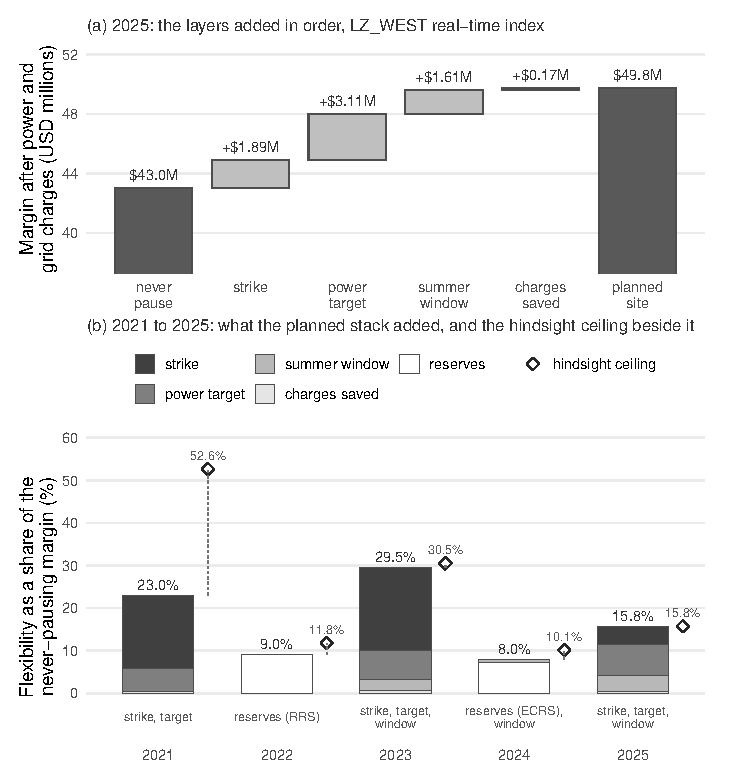
\includegraphics[width=\textwidth]{images/ch9_stack}
  \caption{What the stack was worth, as margin after power and grid charges: mining and reserve revenue, no pool or firmware fee taken out, less the energy and the grid charges. The retail adder, the machines, their depreciation, those fees, site operation, staff and debt are outside the ledger. (a)~2025 as a waterfall: the never-pausing site's margin, then each layer added in the order the chapter stacks them, to the planned site, which in 2025 is also the hindsight ceiling; ``charges saved'' is the losses, ancillary and uplift the paused and underclocked megawatt-hours avoided, plus under \$1,000 of distribution from a lower monthly peak. (b)~2021 to 2025: the value of flexibility to the planned site as a share of the never-pausing site's margin, decomposed along the path it ran. In 2022 and 2024 it had committed both fleets to a reserve award on the previous year's winner, and the reserves segment is Chapter~7's standing revenue. The diamond beside each bar is the hindsight ceiling; in 2021 its 52.6~percent is the RRS award through Uri. The reference site is 67.13~MW (10,000 S19j~Pro and 10,000 S21~XP) at LZ\_WEST, on 15-minute settlement prices and the spliced daily hashprice, with lagged decisions. The planned site commits its reserves each January on the previous year's winner (none in 2021) and calls the summer window on June~1; while it holds reserves, the fleet stays on the meter.} % fig-src: analysis/figures/fig_ch9_stack.R on analysis/data/ch9_optimal_stack.csv (planned 23.0 / 9.0 / 29.5 / 8.0 / 15.8%; hindsight 52.6 / 11.8 / 30.5 / 10.1 / 15.8%, 52.7 and 10.2 until 2026-10-03, when the ledgers booked distribution at $0.50 per MWh consumed); charges saved, 2025: $0.17M (fig_ch9_stack.R console 0.1685) = plan_flex $6,774,783 less strike_gain $1,887,301, tuning_gain $3,112,106 and fourcp_net $1,606,871; its distribution part is ch9_optimal_stack.R console, 2025 DISTRIBUTION and DISTRIBUTION PEAKS lines: never pausing $280,197 billed on 67.13 MW every month, planned $279,261 on monthly peaks of 66.90 MW, 0.23 MW x 1,000 x $0.339183 x 12 = $936; the tuned site's highest quarter-hour is 66.90 MW (S19j Pro 2,700 W + S21 XP 3,990 W a pair) and the never-pausing site is billed on its 67.13 MW nameplate draw, the draw its other charges are booked on, though its energy is priced at the curves' stock points, 67.00 MW, so 0.13 of the 0.23 MW is that booking and 0.10 MW the tuned site's own lower peak; the bill is chapter 6's (analysis/checks/oncor_distribution.R: $0.331004 + $0.008179 per billing kW-month on the month's highest quarter-hour, an 80% ratchet that binds in no month, DISTRIBUTION CHECK line, and $580.43 a month at the one site meter); until 2026-10-03, when the ledgers booked distribution at $0.50 per MWh consumed, the caption counted distribution among the charges a paused megawatt-hour never incurred; the margin basis (EXEC-020): analysis/checks/ch9_optimal_stack.R, total = mining - adders - dist - tcrf + asrev, mining = hashprice x terahash (analysis/data/hashprice_daily_2021on.csv usd_th_day_spliced, no fee deducted) less energy at the settlement price, adders, dist and tcrf the grid charges of chapter 6's tab:btm-ledger (dist since 2026-10-03, when it left the adders); no retail adder (private and excluded, analysis/checks/ch6_btm_ledger.R header), machine, depreciation, fee, site operation, staff or debt line anywhere in the ledger, as chapter-4.tex:77's breakeven ignores the machine, hosting, cooling and staff; the firmware fee, Braiins OS's 2.5% devfee, is priced beside the power target in sec:stack-power-target (ch9_optimal_stack.R FIRMWARE FEE line), not in the ledger; printed as "under $1,000" since 2026-10-03 because $529 of the $936 is the never-pausing site billed on its 67.13 MW nameplate against energy priced at 67.00 MW, and only $407 the tuned site's own lower peak
  \label{fig:stack-shape}
\end{figure}

\begin{table}[tb]
  \centering
  \scriptsize
  \setlength{\tabcolsep}{1.8pt}
  \begin{tabular}{lrrrrrrrr}
    \hline
    \textbf{Year} & \textbf{Never} & \textbf{Strike} & \textbf{Target} & \textbf{Window} & \textbf{Planned} & \textbf{Flexibility} & \textbf{Hindsight} & \textbf{Interf.} \\
     & pause & & & net & site & \$M (\%) & \$M (\%) & \\
    \hline
    2021 & 348.72 & 59.79 & 18.90 & \emph{$-$5.52} & 428.93 & 80.20 (23.0) & 183.60 (52.6) & $-$6.82 \\
    2022 & 132.43 & \emph{6.61} & \emph{7.50} & \emph{1.25} & 144.37 & 11.94 (9.0) & 15.61 (11.8) & $-$1.31 \\
    2023 & 65.49 & 12.73 & 4.41 & 1.75 & 84.78 & 19.29 (29.5) & 19.97 (30.5) & $-$0.67 \\
    2024 & 65.91 & \emph{2.19} & \emph{3.95} & 0.41 & 71.15 & 5.24 (8.0) & 6.68 (10.1) & $-$2.27 \\
    2025 & 43.00 & 1.89 & 3.11 & 1.61 & 49.77 & 6.77 (15.8) & 6.77 (15.8) & $-$1.04 \\
    \hline
    Total & & & & & & 123.46 & 232.63 & \\
    \hline
  \end{tabular}
  \caption{The ledger, in millions of dollars per year, LZ\_WEST real-time index, one engine. ``Never pause'' is the site at stock power in every interval. Strike and power target are margin before grid charges; never pause and planned site are after them, the full transmission charge included. Strike, power target and window are the increments of the price-only stack in that order; italics mark a layer the planned site did not run that year. The planned site sets the two annual switches in advance: reserves in January on the previous year's winner (none in 2021; both fleets on RRS in 2022 and on ECRS in 2024, held on the meter), the window on June~1 by the rule of Section~\ref{sec:stack-peaks} (skipped in 2021 and 2022). Rows do not sum to the planned site: the charges the pauses and power targets saved, up to \$1.5~million a year on the price-only path, are the ``charges saved'' bar of Figure~\ref{fig:stack-shape}. Flexibility is the planned site over the never-pausing one. Hindsight is the hindsight ceiling over the same baseline: RRS for both fleets in 2021 with the window skipped, ECRS in 2023 with the window's hours withheld, the price-only stack otherwise. Interference is the joint price-only stack against the naive sum of strike, power target and the whole transmission prize. Frictionless: Chapter~5's rules cost 0.15~percent of mining margin, before any target move is charged.} % tab-src: analysis/data/ch9_optimal_stack.csv (never_total, strike_gain, tuning_gain, fourcp_net, plan_total, plan_flex, hind_flex, naive_sum, joint_index), written by analysis/checks/ch9_optimal_stack.R; totals from its "Five years" line (planned $123.46M, hindsight ceiling $232.63M); charges saved on the price-only path at most $1.52M (2021: plan_flex $80,204,842 - strike_gain $59,793,587 - tuning_gain $18,895,791 = $1,515,464, of which $1,514,528 losses, ancillary and uplift, never_adders $2,912,565 - plan_adders $1,398,037, and $936 distribution from the lower monthly peak, never_dist $280,197 - plan_dist $279,261, as in the fig:stack-shape caption; until 2026-10-03 the caption called the bar the charges the paused and underclocked megawatt-hours never incurred); no figure in a year's row moved by more than $0.03M on 2026-10-03, when the ledgers stopped booking distribution at $0.50 per MWh consumed and billed it on each month's peak (the totals were $123.51M and $232.69M); frictionless 0.15% and no charge for a power target move in either run, analysis/checks/ch9_control_friction.R; the basis of each column: strike and power target are the L1 and L2 "mining" increments of the ch9_optimal_stack.R console (revenue less energy, before adders, distribution and TCRF; 2025 +$1,887,301 and +$3,112,106), never pause and planned site its grid profit lines, the window its L3 net (after the transmission charge and the other charges its hours avoid), flexibility and hindsight differences of grid profit; until 2026-10-04 the caption said "Every column is margin after power and grid charges", which the next sentences' charges-saved bar contradicted
  \label{tab:stack-ledger}
\end{table}

Read the interference column first. Add the strike, the power-target increment and the whole transmission prize, and 2025 sums to \$7.8~million; the joint price-only stack earned \$6.8~million. The difference is the margin spent emptying the site through 174 window hours the price never flagged, less the charges the strike and power target saved. Adding the layers separately overstates the stack by 15~percent in 2025 and 34~percent in 2024, when two of the four peaks also escaped the window. % src: ch9_optimal_stack.R console, "SUM VS STACK" lines (2025 naive $7,812,221 vs joint $6,774,783; 2024 $8,954,199 vs $6,681,877, interference $2,272,322 of which $1,406,407 is the transmission charge on the two peaks the window missed); on the stack script's stock-power, nameplate basis the 2025 interference is 22% of the naive sum, a 29% overstatement (strike + 4CP only: interference $1,099,208 of a naive $4,927,855; joint $3,828,647); the split of 2025's $1,037,438: the window's margin, TCRF $2,812,814 less its L3 net $1,606,871 = $1,205,943, less the charges the strike and power target saved, plan_flex $6,774,783 - strike_gain $1,887,301 - tuning_gain $3,112,106 - fourcp_net $1,606,871 = $168,505 (fig_ch9_stack.R console, charges saved 0.1685), because the naive sum takes the strike and power target as mining increments, before grid charges, and the joint figure is after them (ch9_optimal_stack.R, the naive and joint lines above its SUM VS STACK print; 2021: $8,336,470 - $1,515,464 = $6,821,006); until 2026-10-04 this line called the whole difference the window's margin
The interference is negative in every year and, in dollars, largest in the storm year, because the strike was highest then and every window hour forgone cost the most.

Then read the two flexibility columns, the plan and the ceiling. On both whole-site rules, the plan and never selling reserves, nearly all of the gap to the ceiling is one January. Graded by capture, as Chapter~5 grades the loop, the planned site earned 88~percent of the ceiling's gain from 2022 to 2025, never selling reserves 96~percent, and both 44~percent in 2021. The planned site earned 23.0, 9.0, 29.5, 8.0 and 15.8~percent more than never pausing from 2021 to 2025, \$123~million more over the five years. The per-fleet rule earned \$112~million more and never selling reserves \$127~million, the other two rules an operator could have set in advance. The hindsight ceiling earned 52.6, 11.8, 30.5, 10.1 and 15.8~percent more, \$233~million. In January 2021 no operator could have known to sell both fleets into RRS, and 2021 alone (the RRS award through Uri less the strike and power target it displaced) is \$103~million of the \$109~million between the two columns. The rest is the two years the plan followed last year's winner into reserves, the one summer its window rule skipped a window that paid, and ECRS's first year, which only hindsight sold. % src: ch9_optimal_stack.R console, CAPTURE line (planned 2021 43.7%, 2022-2025 88.2%; never sell reserves 2021 43.7%, 2022-2025 96.1%; capture as chapter 5 sec:oracle defines it, with the hindsight ceiling as the benchmark; 2021's $103.40M is 94.7% of the planned site's $109.18M gap to the ceiling and 98.2% of never selling reserves' $105.32M), RULES SET IN ADVANCE line ($112.37M old per-fleet rule, $123.46M planned, $127.31M never sell reserves), PLANNED and HINDSIGHT CEILING lines (flexibility over never pausing, 2021-2025: planned 23.0, 9.0, 29.5, 8.0, 15.8%; hindsight 52.6, 11.8, 30.5, 10.1, 15.8%, one decimal as Table 9.2 and the results discussion print them) and the "Five years" line ($123.46M vs $232.63M; 2021 $183.60M - $80.20M = $103.40M of $109.18M; 2022 $3.67M, 2023 $0.67M, 2024 $1.44M, 2025 $0); planned $123.51M, printed $124 million, and hindsight 52.7 and 10.2% until 2026-10-03, when the ledgers booked distribution at $0.50 per MWh consumed; until 2026-10-04 these sentences said the planned site "earned 23.0 ... percent of the never-pausing margin" and the rules and the ceiling "earned" $112M, $127M and $233M: all are flexibility, the gain over never pausing, not what the sites earned (the planned site's own grid profit, PLANNED lines, $428.93M + $144.37M + $84.78M + $71.15M + $49.77M = $779.0M over the five years, 123.0% of the never-pausing margin in 2021)
On reserves the lesson is plain: every time one of those rules said sell, never selling did better, twice for the plan and in all four years from 2022 for the per-fleet rule. Never selling beat the plan by \$3.9~million, but the plan's rule was chosen for what it knew in January, and picking the winner now would be a verdict reached with the five years in hand. Taking the window with hindsight would add \$1.3~million, all of it in 2022; playing the first summer's window, which the rule had no evidence for, would cost \$5.5~million. The plan's one default, for a first January with no previous year, is the one that needs no history: no reserves. Selling RRS that January would have been a lucky guess. Had the site held RRS when Uri arrived, the planned five years would come to \$227~million, within \$6~million of the ceiling, and the companion repository holds no 2020 prices to say which way that January would have gone. % src: ch9_optimal_stack.R console, RULES SET IN ADVANCE line (6 reserve commitments, planned 2 and old per-fleet rule 4; never selling reserves better in all 6, by $1.44M to $5.54M) and the two "differs from never selling reserves" lines (planned 2022 -2.41M, 2024 -1.44M; old per-fleet rule 2022 -2.41M, 2023 -5.54M, 2024 -3.14M, 2025 -3.85M); five-year alternatives line (never sell reserves $127.31M; old per-fleet rule on last year's data $112.37M; planned reserves, window in hindsight $124.78M; planned with the first summer's window played $117.93M; against planned $123.46M) and first-year default line ($226.85M with 2021 on RRS; ceiling $232.63M)
Chapter~2's week in February is where nearly half of the five-year value of flexibility to the planned site was earned, by pausing through the storm, and seven tenths of what the hindsight ceiling would have paid, on the reserve convention that books its RRS award. % src: analysis/checks/ch9_optimal_stack.R console, STORM SHARE line (Feb 14-20, 2021: $58.62M of the planned five-year $123.46M = 47%; $166.87M of the hindsight five-year $232.63M = 72%)

Per megawatt-hour the site consumed at stock, flexibility was worth \$137 to the planned site in 2021, \$20 in 2022, \$33 in 2023, \$9 in 2024 and \$12 in 2025; the ceiling's \$313 in 2021 is the reserve award. % src: ch9_optimal_stack.R console, PLANNED lines ($136.76 / $20.31 / $32.81 / $8.89 / $11.52 per MWh of 586,448 / 588,059 / 588,059 / 589,670 / 588,059 MWh; the PER MWh lines' "flexibility earns ... per MWh consumed at stock as planned") and the 2021 HINDSIGHT CEILING line ($313.07); until 2026-10-04 this line said "the planned site earned $137 in 2021 ...", the gain over never pausing, not its margin, which was $731 per MWh in 2021 ($428,927,595 / 586,448 MWh)
And the charges the grid site paid on top of energy fell from \$7.94 per megawatt-hour when it never paused to \$3.08 for the planned site in 2025, almost all of it because the window removed the transmission charge. The loss, ancillary and uplift charges left with the paused and underclocked megawatt-hours, so per megawatt-hour they hardly changed. The distribution bill barely moved: the wires utility charges it on each month's highest quarter-hour, as Chapter~6 noted, so a pause avoids it only where it lowers that month's peak. % src: ch9_optimal_stack.R console, "PER MWh" line 2025 (never-pause $7.94; planned $3.08; the $4.86 fall is $4.78 of transmission, TCRF $2,812,814 / 588,059 MWh never pausing and none planned; losses, ancillary and uplift $2.68 per MWh never pausing, never_adders $1,575,335 / 588,059 MWh, and $2.56 planned, plan_adders $1,379,207 over the 539,189 MWh drawn, (plan_adders + plan_dist) / charges_per_mwh_plan, analysis/data/ch9_optimal_stack.csv; until 2026-10-03 the sentence credited the pauses and underclocking with removing those charges with the megawatt-hours, true of the dollars, not of the rate; $7.96 and $3.06 until 2026-10-03, when the ledgers booked distribution at $0.50 per MWh consumed, which the pauses appeared to remove with the megawatt-hours) and the 2025 DISTRIBUTION line (never pausing $280,197, planned $279,261, $936 apart: $0.476 and $0.518 per MWh consumed, nearly the same bill over fewer megawatt-hours); planned monthly peaks 66.90 MW in every month of 2025 (DISTRIBUTION PEAKS line), so no pause lowered one; the bill is chapter 6's, analysis/checks/oncor_distribution.R (oncor2026retailtariff sec. 6.1.1.1.7, Transmission Service, as chapter-6.tex:74 quotes it: $0.331004 Distribution System Charge + $0.008179 Rider DCRF per billing kW-month on the month's highest 15-minute NCP with an 80% ratchet, plus $258.80 customer and $321.63 metering per meter-month)

\begin{figure}[htbp]
  \centering
  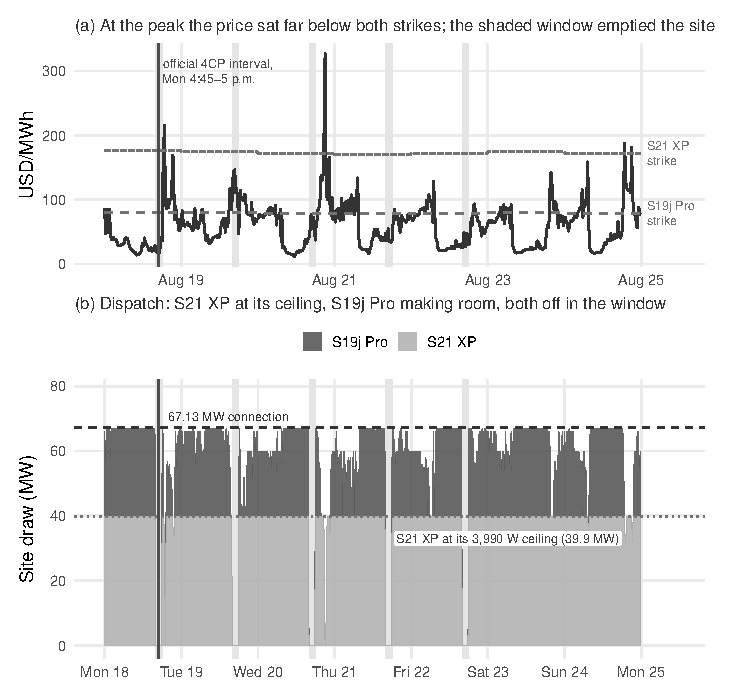
\includegraphics[width=\textwidth]{images/ch9_dispatch_week}
  \caption{One summer week, two fleets, one connection: August 18 to 24, 2025, at LZ\_WEST, the week that holds the month's official 4CP interval. (a)~The settlement price against the two strikes; the price never reached the S19j~Pro's strike in the official interval, which the summer window (shaded) caught anyway. (b)~The dispatched megawatts: the S21~XP pinned at its 3,990~W ceiling through 92~percent of the week, the S19j~Pro running below stock to make room under the connection for 85~percent of it and off for 15~percent, six points of it in the window, when both fleets were dark. At stock power the fleets would draw 30.68~MW (S19j~Pro) and 36.45~MW (S21~XP).} % fig-src: analysis/figures/fig_ch9_dispatch_week.R on analysis/data/ch9_dispatch_week_2025.csv (ch9_optimal_stack.R console: window applied as the planned site plays it; site mean 57.4 MW; S21 XP at ceiling 92%; S19j Pro below stock but on 85%, off 15%, window 6% of the week)
  \label{fig:stack-week}
\end{figure}

Figure~\ref{fig:stack-week} shows the stack physically, in one August week of 2025. The efficient fleet sits at its ceiling almost every quarter-hour. The old fleet runs below stock to fit under the connection and switches off only when the price climbs well past its strike. On Monday afternoon the summer window empties the site while the price, at about \$18 in the quarter-hour ending at 5~p.m., is nowhere near either strike, and that quarter-hour turns out to be the month's official peak. % src: analysis/data/ch9_dispatch_week_2025.csv (official interval 2025-08-18 16:45-17:00, ERCOT label 17:00, at $17.76/MWh; strikes about $79 / $173 that week); ch9_optimal_stack.R console, dispatch week line; the old fleet on the loop's last settlement price, the same csv: outside the window off in 59 quarter-hours, every one after a price of $97.80 or more, at least 1.24 times strike19 ($77.85 to $80.66 that week, the nameplate strike panel (a) draws), and on at 12 to 20 MW in 95 quarter-hours after the price had passed strike19, up to $100.55, against 20 to 27 MW below it; 29.5 / 23.83 = 1.24, the breakeven at its most efficient power target (ch9_flexibility_stack.R console, Layer 4: best 23.83 J/TH at 1200 W; sec:stack-power-target); until 2026-10-04 this line said it "switches off when the price climbs toward its strike"

The strategy, then, is an order of switching, which Section~\ref{sec:stack-rule} states as a procedure. Inside the year it runs with no look-ahead at all. The two annual switches are the only choices the ledger could have made with hindsight, and the headline sets them in advance.

\section{The Other Offer: Behind the Fence}
\label{sec:stack-fence}

Now the second document on the desk. Section~\ref{sec:btm} set the terms: nearly \$9 per megawatt-hour of charges on top of energy, of which a site that dodges the four peaks already escapes about \$5.70, so the fence saves about \$3 against that competent neighbor; the real prize sits on the energy line, between the generator's captured price near \$19 and, on the hours the wind blew, a grid price near \$40. The fence priced here is firm and delivers flat, and for a flat load the grid alternative with the peaks dodged is the \$45 of Chapter~6's table, so the prices tested run from \$19 to \$45. The same section added that an islanded mine forfeits every layer this chapter has just priced. This section prices the forfeit. % src: chapter 6 tab:btm-ledger and sec:btm (analysis/checks/ch6_btm_ledger.R console: energy 42.18; stack 8.83; TCRF 5.65; residual 3.18 islanded; delivered 51.01 / 45.35 flat; top of band 39.90 on wind hours); ch9_optimal_stack.R BAND (19, 45)

The comparison is built on the same engine, with every assumption stated. Both sites use the same fleet and 67.13~MW power budget, with lagged decisions over the same five years. The fenced site pays one negotiated price for every megawatt-hour and nothing else: no losses, no ancillary or uplift allocation, no transmission charge, and, with no grid tie and so no utility meter, no distribution line. It sells no reserves, dodges no peaks, arbitrages no index, and it moves its power targets against its fixed price like anyone else, because the target is firmware. The ledger treats its plant as always available, a gas plant or a firmed contract; a wind-only island would run only when the wind blew, and Chapter~6 already noted that it is least covered at 5~p.m.\ in August. The ledger prices two behaviors of the generator. Under \glossaryterm{firm-supply}{firm supply} the mine runs whenever it wants. Under an \glossaryterm{interruptible}{interruptible} deal the generator keeps the right to switch the mine off whenever the grid pays more than the mine does, sells into the grid instead, and pays the mine nothing for the interruption. The zone price stands in for the plant's node price, which sits lower in West Texas, so the interruptions are overstated. % src: analysis/checks/ch9_optimal_stack.R header (behind-the-meter design; no distribution because it is chapter 6's islanded case, with no grid tie and no utility meter to bill, chapter-6.tex:74 and :80) and console
The question for each year is the \glossaryterm{indifference-price}{indifference price}: the negotiated price at which the fenced site earns exactly what the grid site earns. Below it the fence wins; above it the grid does.

\begin{table}[htbp]
  \centering
  \scriptsize
  \setlength{\tabcolsep}{1.6pt}
  \begin{tabular}{lrrrrrrrrr}
    \hline
    \textbf{Year} & \textbf{Grid,} & \textbf{Grid,} & \multicolumn{3}{c}{\textbf{Fence, firm, at}} & \textbf{Runs at} & \multicolumn{3}{c}{\textbf{Indifference price vs.}} \\
     & never pause & planned & \$19 & \$30 & \$45 & \$45, int. & planned & hindsight & never \\
    \hline
    2021 & 348.72 & 428.93 & 449.71 & 443.28 & 434.52 & 83\% & 54.56 & none & 191.80 \\
    2022 & 132.43 & 144.37 & 170.41 & 163.96 & 155.17 & 51\% & 63.44 & 57.17 & 84.09 \\
    2023 & 65.49 & 84.78 & 98.71 & 92.26 & 83.47 & 76\% & 42.76 & 41.62 & 75.88 \\
    2024 & 65.91 & 71.15 & 84.35 & 77.88 & 69.08 & 77\% & 41.46 & 39.00 & 50.43 \\
    2025 & 43.00 & 49.77 & 64.45 & 58.00 & 49.23 & 63\% & 44.06 & 44.06 & 55.89 \\
    \hline
  \end{tabular}
  \caption{Grid versus fence, millions of dollars per year and \$/MWh. The grid columns repeat the never-pausing and planned sites of Table~\ref{tab:stack-ledger}. The fence columns are the same fleet behind a firm generator at three negotiated prices, power targets free on both sides. ``Runs at \$45, int.'' is the share of quarter-hours an interruptible deal at \$45 would have left the mine running. The indifference price is the firm price at which the fence matches the grid site: against the planned site, against the hindsight ceiling, and against the never-pausing site; ``none'' means no positive price would do. Biases, each stated with its direction: firm always-available supply favors the fence; the zone price as the generator's alternative overstates interruptions; the 2025 charges held for every year flatter the grid site in 2021 to 2023, when allocations were higher; the fence's interconnection, study and legal costs fall on its discount and are not priced.} % tab-src: analysis/data/ch9_btm_indifference.csv (references planned, hindsight, never; firm) and ch9_optimal_stack.csv, written by analysis/checks/ch9_optimal_stack.R; run shares from its console ("interruptible runs" at P = $45: 83% / 51% / 76% / 77% / 63%)
  \label{tab:stack-fence}
\end{table}

\begin{figure}[htbp]
  \centering
  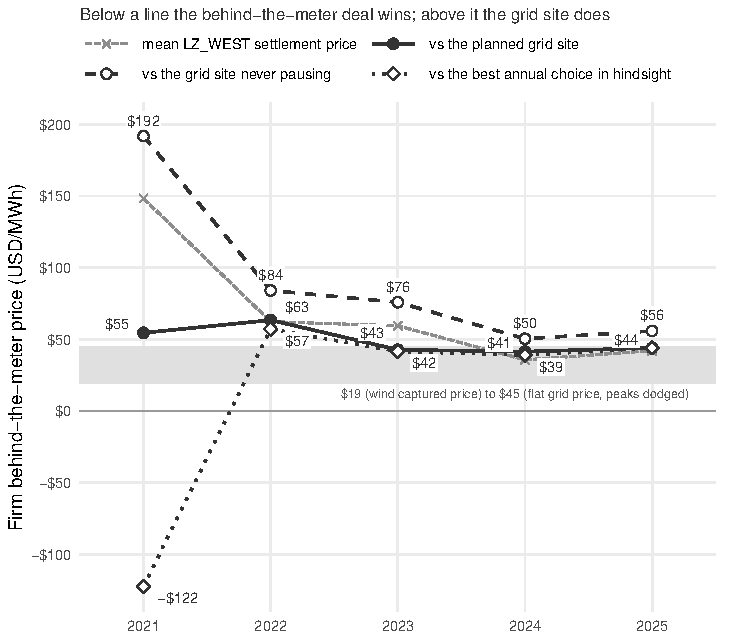
\includegraphics[width=\textwidth]{images/ch9_btm}
  \caption{Where the fence breaks even. The firm negotiated price at which a behind-the-meter site earns what the grid site earns, year by year, against the planned site (solid), against the hindsight ceiling (dotted) and against the same site never pausing (dashed); the mean LZ\_WEST settlement price for reference; shaded, the prices tested, from the wind captured price to the flat grid price with the peaks dodged. Both sites run the same 67.13~MW fleet and power budget, with power targets free on both sides; the behind-the-meter site pays no losses, ancillary, uplift, distribution or TCRF charges and sells no reserves. The planned grid site sets its annual switches in advance. Only the hindsight ceiling of 2021, a grid site that sold RRS through the February storm, has no positive answer.} % fig-src: analysis/figures/fig_ch9_btm.R on analysis/data/ch9_btm_indifference.csv
  \label{fig:stack-btm}
\end{figure}

The comparison in Table~\ref{tab:stack-fence} and Figure~\ref{fig:stack-btm} depends on the grid-site baseline. Against the never-pausing grid site the fence wins at any price in the range in every year: the indifference prices are \$192, \$84, \$76, \$50 and \$56, all above its top, as expected of a site that pays every spike and every peak and never moves its power target. Against the planned site the fence also wins everywhere in the range in 2021 and 2022, where the indifference prices are \$55 and \$63. In 2023, 2024 and 2025 they are \$43, \$41 and \$44, near its top, so a firm deal in the twenties or thirties still beats the stack and one at \$45 does not. Only the hindsight ceiling puts the storm year out of reach: the fence would have had to be paid \$122 for every megawatt-hour it took to match a site that sold reserves through Uri. Against the ceiling the other four years sit at most \$6 lower, at \$57, \$42, \$39 and \$44. % src: analysis/data/ch9_btm_indifference.csv (firm: 54.56, 63.44, 42.76, 41.46, 44.06 vs planned; -122.35, 57.17, 41.62, 39.00, 44.06 vs hindsight; 191.80, 84.09, 75.88, 50.43, 55.89 vs never); the never-pausing site's delivered price, ch9_optimal_stack.R console PER MWh lines, mean energy price plus its charges (it draws flat, so it pays the time-weighted mean): 148.33 + 10.24, 62.35 + 8.37, 59.42 + 8.31, 35.71 + 7.78 = $43.49 in 2024 and 42.18 + 7.94 = $50.12 in 2025; 2024 at $45 the firm fence earns $69,078,122 against never pausing's $65,911,448 (+4.8%, the "at P = $45" line), but at stock power it would trail: revenue before energy $91,519,083 (2024 FIRMWARE FEE line) less 45 x 588,528 MWh (67.00 MW at the curves' stock points x 8,784 h) = $65.04M; until 2026-10-04 this line said the never-pausing site "pays a delivered price above $45" in every year
In 2022, 2024 and 2025 a firm price in the twenties or low thirties beats everything the grid site can plan with its switches, because the stack was worth \$9 to \$20 per megawatt-hour and the discount below the zone price plus the avoided charges was worth more. In the storm year the planned site's stack was worth \$137 per megawatt-hour on a \$148 average price, and a firm fence at \$45 still beat it, because a firm deal buys Uri's week at \$45, the first of the biases the table's caption names. Only the reserve award of the hindsight ceiling, \$313 per megawatt-hour, put the grid site beyond any discount. % src: ch9_optimal_stack.R console, PLANNED lines (flexibility per MWh: 2022 $20.31, 2024 $8.89, 2025 $11.52; 2021 $136.76), 2021 HINDSIGHT CEILING line ($313.07) and mean price (2021 $148.33); 2021 firm BTM profit at $45 $434,517,092 vs planned grid $428,927,595; until 2026-10-04 this line said "the planned site earned $137 per megawatt-hour", its flexibility, not its margin, which was $731 per MWh ($428,927,595 / 586,448 MWh)
The fence is an annuity: a discount on every megawatt-hour, the same in a storm as on a Tuesday in April. The stack is an option: thin most of the time, and worth years of the annuity in Uri's week, under a cap since lowered (Section~\ref{sec:ordc}).

The second finding is about the switch, not the price, and it is the reason the firm case is a ceiling. An interruptible fence, where the generator takes the power back whenever the grid pays more than the mine does, matches the planned site at no price in any of the five years. At \$19 in 2025 such a mine would have run 24~percent of the year; at \$45, 63~percent; the best it could do at any price, about \$32~million at a price near \$55, is a third short of the grid site's \$50~million. % src: ch9_optimal_stack.R console, "interruptible" lines (matches the planned grid site up to P = no price in every year; 2025 runs 24% at $19, 45% at $30, 63% at $45; best case $31,954,770 at P = $55; planned grid $49,772,629)
Every hour the grid pays more than the contract is an hour the fenced mine goes dark for nothing: every hour in which the grid site's pause is worth money, and every hour between the contract price and the strike in which the grid site mines at a profit. The sell option Chapter~6 valued in Section~\ref{sec:ownergen}, about \$960,000 per megawatt-year for the S19j~Pro in 2021 and \$51,000 in 2025, has moved to the generator's side of the fence. % src: analysis/checks/sell_vs_mine.R console, moving-strike table (2021 $957,665; 2025 $51,499 per MW-yr), as quoted in chapter 6 sec:ownergen, the S19j Pro's; the S21 XP's same-interval option was smaller, 31,320,751 / 36.45 MW = $859,280 and 675,521 / 36.45 = $18,533 per MW-yr (ch9_flexibility_stack.R console, "The price of not seeing the future", foresight gains); until 2026-10-04 this line named no fleet
A generator that keeps the switch sells the mine electrons and keeps the option; a mine that keeps the switch sells its flexibility to the grid.
Firmness matters alongside price in a behind-the-meter deal. A firm price in the lower half of the \$19 to \$45 range beat the planned site in every one of the five years, and firmness through a storm week is exactly what no generator gives away at \$45. % src: analysis/data/ch9_btm_indifference.csv (firm BTM profit at $19 and $30 above the planned grid site in every year; the 2021 row above)

The filings show what the industry has concluded from the same arithmetic, and it is neither pure case. Hut~8's Vega site runs behind a wind farm and in front of the grid at once; Soluna's Dorothy sits behind a plant it does not own and still earned demand-response revenue; Riot's fixed-price contracts with sell-back rights produced \$54~million of curtailment credits in 2025. % src: chapter 6 sec:btm (hut8_10k2025; soluna10k2025 $1.285M; riot10k2025 $54.302M manual curtailment credits)
The hybrid buys the annuity and keeps the option. The companion repository holds no generator-availability data, so the hybrid is described here and not modeled; its economics are, at best, the firm fence's margin in Table~\ref{tab:stack-fence} plus the strike and any reserves, the two layers only a grid tie adds, less whatever the generator charges for letting the mine keep its switch. % src: tab:stack-fence fence columns (power targets free on both sides; no transmission charge, so the summer window has nothing left to save); until 2026-10-04 this line added "the planned site's flexibility and the firm fence's discount from Table 9.3", a discount the table does not print, whose natural reading, a fence column less the never-pausing one, already holds the fence's own power target, and whose energy and charges include the transmission charge the flexibility's window also counts (2025 at $45: fence $49.23M less never pausing $43.00M = $6.23M, about $3.0M of it the discount, (42.18 + 7.94 - 45) x 588,059 MWh, ch9_optimal_stack.R console PER MWh line, and about $3.2M the power target)

\section{The Decision Rule}
\label{sec:stack-rule}

% layout (2026-10-05): this, the \looseness on step 7 and the enlargement before "The parts were worth less" keep chapter 9's last lines off a page of their own; revisit if the text above changes
\enlargethispage{2\baselineskip}
For a site of your own, the chapter reduces to eight steps.

\begin{enumerate}
  \item Compute each machine model's strike every day: yesterday's hashprice times 41,667, divided by the model's joules per terahash.
  \item Keep the pause alive: take-or-pay without resale only at a discount above the flexibility lost. If you index, index real time.
  \item Run one strike per model with the three rules of Chapter~5. Never blend the fleets into one site strike.
  \item Move the power target, and size the connection just under 75~MW, counting every load at the site. % src: sec:stack-power-target, the design-brief sentence (75 / 1.10 = 68.18 MW of machines at most, chapter-1.tex PUE 1.10; this fleet's full tilt 74.10 MW, 81.5 MW at the meter); until 2026-10-04 this step said "size the connection for full tilt below 75 MW", written when the brief sized the connection for the machines alone (PER-3 moved the brief to every load at the meter and left "for full tilt" here)
  \item Decide the summer window on June~1. Play it only if your fleet's power-weighted margin, the strike on yesterday's hashprice less last summer's window price, is under the transmission prize divided by the window's hours. Budget no transmission saving before the year after a new site's first full summer: until then the wires utility bills it on an estimate \autocite{oncor2026retailtariff,centerpoint2026retailtariff}. Never sell the emergency program's afternoon block.
  \item Decide reserves interval by interval, through your load resource's QSE (Chapter~7). Under RTC+B a day-ahead award can be bought back at the real-time reserve price. When the price beats your strike by more than that buyout, telemeter your reserve away, then pause once the five-minute run stops awarding it. Never sell the window's hours. Expect little: every rule set in January that said sell lost to never selling.
  \item \looseness=-1 Take a fence offer only if it is firm and its price is below the indifference price your own numbers produce. Walk away if the generator keeps the right to interrupt without paying for it, or if the deal islands the site; a fence with a grid tie is the hybrid of Section~\ref{sec:stack-fence}. Clear the netting rules of Section~\ref{sec:btm} before you sign.
  \item Run the calculator in the companion repository for your zone and contract, with your fleet as a mix of its two machines, and read the friction line in its footer.
\end{enumerate}

% layout (2026-10-04): lets the chapter's last page run long so its final lines do not spill onto a page of their own; move or drop if the text above changes
\enlargethispage{3\baselineskip}
The parts were worth less together than a brochure would add them up to. The size of the prize was set by hashprice and the market's regime, not by the grid's generosity.

Three things move after the data ends, and Chapter~10 takes them up. RTC+B, which step~6 already assumes, turns reserves into a priced option rather than an either/or. 12CP and the minimum billing demand, if adopted as proposed, would shrink or end the peak layer. And hashprice, which sets every threshold in this chapter, rests on a subsidy that halves on a schedule.
